\documentclass[journal]{IEEEtran}
\usepackage{cite}
\usepackage{amsmath,amssymb,amsfonts}
\usepackage{graphicx}
\usepackage{textcomp}
\usepackage{xcolor}
\usepackage{hyperref}
\usepackage{algorithm}
\usepackage{algpseudocode}
\usepackage{booktabs}
\usepackage{caption}
\usepackage{float}

\hypersetup{
    colorlinks=true,
    linkcolor=blue,
    filecolor=magenta,      
    urlcolor=cyan,
}

\begin{document}

\title{Dynamic Hybrid Forecasting Models for Drug Consumption Prediction in Hospital Pharmacies}

\author{Yuxin Fan$^{*}$ and Siye Wu$^{\dagger}$ \\
$^{*}$School of Engineering and Applied Science, University of Pennsylvania, Canada, Toronto \\
Email: yuxinfan@alumni.upenn.edu \\
$^{\dagger}$Simon Business School, University of Rochester, Canada, Toronto \\
Email: april.siyewu@hotmail.com}

\maketitle

\begin{abstract}
Efficient and accurate drug consumption forecasting is important for hospital pharmacies to avoid overstocking, minimize wastage, and ensure continuous patient care. This study introduces a hybrid forecasting framework integrating XGBoost, Prophet, and SARIMAX to improve monthly consumption predictions at the drug-manufacturer level. Through rolling-window forecasting and advanced feature engineering, the proposed approach fixes challenges such as seasonality, trend shifts, and sparse data. The model results show improvements in prediction accuracy and robustness across drug consumption scenarios.
\end{abstract}

\begin{IEEEkeywords}
Drug Consumption Forecasting, Hospital Pharmacies, Forecasting Models, XGBoost, Prophet, SARIMAX
\end{IEEEkeywords}

\section{Introduction}

Drug consumption forecasting is critical in hospital pharmacy inventory management. Accurate drug consumption predictions enable hospital pharmacies to ensure drug availability while minimizing costs associated with overstocking or stockouts. As highlighted by Koala et al.~\cite{koala2021factors}, forecasting drug consumption is very challenging due to numerous influencing factors, such as sociodemographic characteristics, morbidity patterns, drug price index, and seasonal reasons like disease outbreaks or policy changes, resulting in highly complex and dynamic consumption patterns. Therefore, the purpose of our study is to integrate a hybrid framework combining machine learning and statistical methods to enhance drug consumption forecasting for hospital pharmacies.

Taylor and Letham~\cite{taylor2018forecasting} introduced Prophet, a scalable forecasting method designed for large-scale applications, which excels at capturing general trends and seasonality through changepoint detection. While Prophet is effective in many scenarios, it often requires dedicated tuning to prevent overfitting to localized patterns and has limited capability in incorporating external variables. Extreme Gradient Boosting (XGBoost), proposed by Chen and Guestrin~\cite{chen2016xgboost}, has demonstrated great success in applications such as sales prediction and customer behavior modeling, highlighting its flexibility across diverse domains. When used in scenarios such as tracking drug consumption patterns over time, XGBoost's effectiveness may be reduced with limitations in capturing sequential dependencies in time-series data.

More models were introduced to address some of the above limitations. Meng et al.~\cite{meng2021comparative} introduce that models like Long Short-Term Memory (LSTM) excel in drug sales forecasting by capturing long-term dependencies and non-linear patterns, while Prophet effectively handles seasonality and holiday effects. However, LSTM requires high computational resources, and Prophet's reliance on trend assumptions can limit adaptability in dynamic environments affected by policy changes or disease outbreaks. Xu et al.~\cite{xu2019hybrid} propose a hybrid approach that combines a linear regression (LR) model, specifically the auto-regression (AR) or auto-regressive integrated moving average (ARIMA) model, and a deep belief network (DBN) to improve time series forecasting by capturing both linear and nonlinear patterns. While this method demonstrates high accuracy in general time series prediction, it relies on computationally intensive DBN training and limited consideration of irregular external factors. Siddiqui et al.~\cite{siddiqui2021hybrid} propose a mixed forecasting model, ARIMA-Holt’s Winter (ARHOW), which combines the strengths of the ARIMA model and the Holt-Winters method to enhance forecasting accuracy. Relying on fixed model architectures and pre-set parameters sometimes can limit its adaptability in the dynamic pharmaceutical industry. Rathipriya et al.~\cite{rathipriya2022pharma} develop a hybrid demand forecasting model using both shallow neural networks like Radial Basis Function Neural Network (RBF\_NN) and Generalized Regression Neural Network (GR\_NN), and deep learning models like LSTM and Stacked LSTM to predict pharmaceutical sales. Their study shows that shallow neural network handle smaller datasets and noise effectively, while shallow networks handle small datasets and noise well, deep learning models capture non-linear and temporal patterns more effectively but require significant computational resources and large datasets.

In our study, we analyze monthly drug consumption data collected from hospital pharmacies over nearly seven years, covering a wide range of drugs and manufacturers. This dataset exhibits high variability, influenced by factors such as seasonality, external policy changes, and irregular demand patterns. Given these complexities, no single forecasting method can effectively address all aspects of drug consumption prediction. 

To address this, we propose DynamicXSP, a hybrid model integrating Prophet, SARIMAX, and XGBoost. Besides, by leveraging rolling-window forecasting, feature engineering, and grid search, DynamicXSP combines the strengths of each method to effectively capture long-term trends, external influences, and non-linear dependencies, providing a more comprehensive solution for drug consumption forecasting. In details, Prophet captures long-term trends and seasonality, SARIMAX adjusts for external influences and short-term fluctuations, and XGBoost models non-linear dependencies and sparse observations.

The remainder of this paper is arranged as follows: Section II introduces the research methodology and focuses on the advantages of the DynamicXSP framework. Section III presents the experiments and results, including data preprocessing and analysis. Finally, Section IV summarizes the study and outlines future directions on research.

\section{Methodology}
\subsection{DynamicXSP Model Framework}

 DynamicXSP follows a structured process:

\begin{itemize}
    \item Model training applies multiple models like SARIMAX, XGBoost and Prophet with automating grid search and rolling-window forecasting to ensure adaptability to recent trends.
    \item Feature engineering includes rolling statistics, lag-based variables and external factor indicators to enhance predictive modeling.
    \item Model selects the best one from multiple models based on the performance metrics such as \( R^2 \) and symmetric Mean Absolute Percentage Error (SMAPE).
\end{itemize}

\begin{figure}[H]
    \centering
    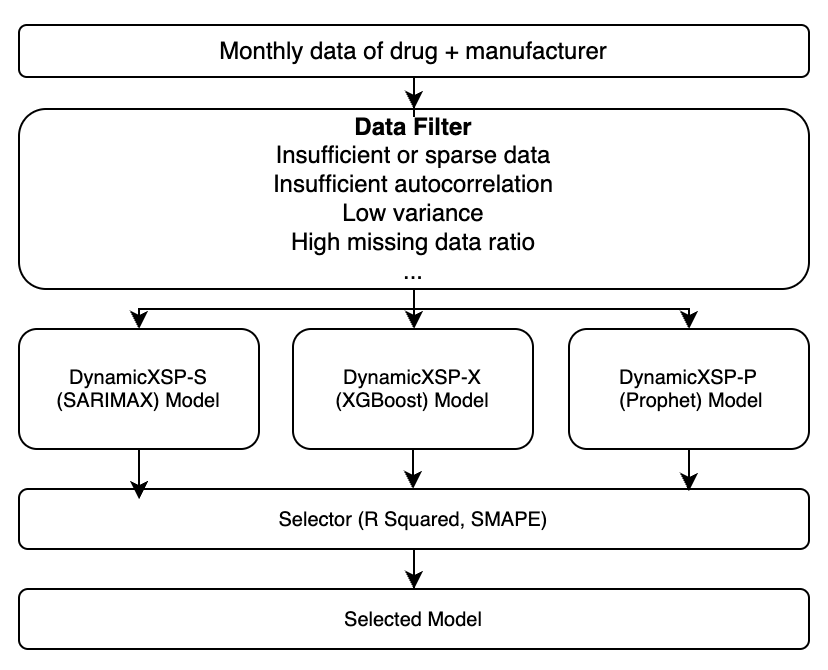
\includegraphics[width=\linewidth]{./model_structure.png}
    \caption{Model Structure of DynamicXSP Framework}
    \label{fig:vitaminb1}
\end{figure}

\subsection{Model Design and Roles}
\subsubsection{DynamicXSP-S (SARIMAX) Model}

This approach considers not only historical trends but also external influences such as manufacturer supply patterns and drug inventory policies at hospital. The model is defined as below:

\begin{equation}
    \hat{y}_{t} = \phi(B)\theta(B)^{-1} \left( c + \mathbf{X}_{t}\beta + \epsilon_{t} \right),
\end{equation}

where \(y_{t}\) represents the weekly drug inventory consumption, \(\mathbf{X}_{t}\) represents the set of exogenous features designed to capture the relevant consumption patterns, and \(\epsilon_{t}\) is a white noise error term.

To improve prediction accuracy, the DynamicXSP-S model includes specific feature engineering tailored to hospital pharmacy demand. These features take both short-term fluctuations and long-term trends, improving the adaptability of the model in dynamic environments. The main engineered features include:

\begin{itemize}
    \item Lagged value: captures the delayed effect of past consumption, especially suitable for modeling hospital replenishment cycles and manufacturer supply constraints:
    \begin{equation}
    \text{drug\_consume\_lag}_{k} = y_{t-k}, \quad k \in \{1, 3, 6, 12\}.
    \end{equation}
    The lag selections is consistent with common drug purchase intervals in historical data.

    \item Rolling statistics: represent short-term demand fluctuations and variations and help the model explain unexpected spikes in drug use due to policy changes or seasonal illnesses:
    \begin{align}
    \text{consume\_rolling\_mean}_{k} &= \frac{1}{k} \sum_{i=1}^{k} y_{t-i}, \\
    \text{consume\_rolling\_std}_{k} &= \sqrt{\frac{1}{k} \sum_{i=1}^{k} (y_{t-i} - \text{mean})^2}.
    \end{align}
    Unlike standard moving averages, these rolling features are dynamically adjusted to ensure adaptability across different drug types and manufacturers.

    \item Seasonality encoding: Due to hospital procurement schedules, drug consumption often follows predictable monthly cycles. To simulate this effectively, we employ trigonometric transformations:
    \begin{align}
    \text{month\_sin} &= \sin\left(\frac{2\pi \cdot \text{month}}{12}\right), \\
    \text{month\_cos} &= \cos\left(\frac{2\pi \cdot \text{month}}{12}\right).
    \end{align}
    This formulation enables SARIMAX to smoothly capture periodic fluctuations without manually performing seasonal differencing.

    \item Exponentially Weighted Moving Average (EWMA): Introduces a memory-adjusted smoothing technique that prioritizes recent observations, making the model more responsive to sudden shifts in drug demand:
    \begin{equation}
    \text{EWMA}_{\alpha} = \alpha y_{t} + (1-\alpha) \cdot \text{EWMA}_{\alpha,t-1}.
    \end{equation}
    The smoothing factor \(\alpha\) is adjusted according to the specific volatility of drug (in our model, we use 3), to ensure that short-term demand peaks are reflected in the model while filtering out noise.

    \item Percentage change and trend strength: Designed to measure relative variations and stability in consumption patterns, providing key signals for adaptive inventory planning:
    \begin{align}
    \text{pct\_change\_consume}_{k} &= \frac{y_{t} - y_{t-k}}{y_{t-k}}, \\
    \text{comsume\_trend\_strength} &= \frac{1}{k} \sum_{i=1}^{k} \lvert y_{t-i} - y_{t-i-1} \rvert.
    \end{align}
    The trend strength metric allows the model to differentiate between regular seasonal variations and abrupt changes due to supply chain disruptions.
\end{itemize}

These features were selected through statistical analysis of hospital pharmacy consumption data, ensuring that the SARIMAX model effectively captures both recurring demand patterns and unexpected fluctuations. By incorporating rolling-window forecasting and dynamically adjusting feature selection for each drug-manufacturer pair, our approach improves predictive accuracy and enhances robustness in real-world hospital inventory management.

\subsubsection{DynamicXSP-X (XGBoost) Model}

XGBoost is a gradient boosting framework that constructs an ensemble of decision trees to predict the target variable \(y_t\). IIt excels in time-series forecasting, particularly for data with non-linear relationships and sparsity, making it well-suited for predicting drug consumption, where demand varies across manufacturers and fluctuates due to external factors. The model predicts \(y_t\) through an additive function:

\begin{equation}
\hat{y}_{t} = F(x_{t}) = \sum_{k=1}^{K} f_{k}(x_{t}), \quad f_{k} \in \mathcal{F},
\end{equation}

where \(\hat{y}_{t}\) is the predicted value, \(x_{t}\) represents input characteristics, \(f_{k}\) represents the \(k\)-th decision tree, and \(\mathcal{F}\) is the space of decision trees.

To effectively model time dependencies, the DynamicXSP-X framework incorporates lagged values (\(y_{t-1}, y_{t-2}, \dots\)), rolling statistics (such as moving averages and standard deviations over 3, 6, and 12 periods), and indicators reflecting consumption trends. These engineering features enable the model to identify historical patterns of drug usage and detect changes in demand, which is crucial given the variation across manufacturers. Additionally, the interaction terms between lagged values and rolling statistics further enhance the ability of the model to capture advanced dependencies.

The key hyperparameters, including the number of estimators, tree depth, learning rate and sampling ratios, are optimized by grid search to strike a balance between accuracy and computational efficiency. As part of the hybrid forecasting framework, DynamicXSP-X continuously updates its training data, ensuring adaptability to changing demand patterns.

DynamicXSP-X complements statistical models like DynamicXSP-S by capturing non-linear interactions and irregular consumption trends. It is able to learn intricate patterns from historical data, making it a adaptive and robust component in the prediction system.

\subsubsection{DynamicXSP-P (Prophet) Model}

Prophet is a time-series forecasting model, designed to decompose data into trend, seasonality, and external event components. In our model, we optimized Prophet to DynamicXSP-P to make it more effective for handling missing values, outliers, and irregular consumption patterns for drug demand forecasting, where sudden fluctuations and manufacturer-specific trends are common. The model predicts the target variable \(y_t\) as:

\begin{equation}
y_{t} = g(t) + s(t) + h(t) + \epsilon_{t},
\end{equation}

where \(g(t)\) represents a long-term trend, \(s(t)\) captures seasonal patterns using Fourier series, \(h(t)\) considers external disturbances (such as supply chain delays or regulatory policy changes), and \(\epsilon_{t}\) is the white noise error term. This decomposition enhances interpretability while allowing the model to dynamically adjust to various consumption behaviors.

The key hyperparameters are optimized to ensure that the model can effectively adapt to changes in drug demand. The adjustment process focuses on:
\begin{itemize}
    \item \textit{seasonality\_mode}: Determines whether seasonal effects are additive or multiplicative, based on consumption volatility.
    \item \textit{changepoint\_prior\_scale}: Controls the sensitivity to sudden trend changes, which are essential to model demand surgency or supply disruptions.
    \item \textit{seasonality\_prior\_scale}: Adjusts the weights of seasonal components to ensure a balance between smooth short-term variations and long-term trends.
\end{itemize}
The higher \textit{changepoint\_prior\_scale} value allows the model to react more quickly to structural changes, such as increased demand due to new hospital procurement policies, while lower values favor smoother trend transitions.

DynamicXSP-P benefits from continuous data updates, allowing it to react responsive to changing drug consumption trends while preventing overfitting outdated patterns. Through leveraging decomposition-based prediction and hyperparameter tuning, Prophet provides an interpretable prediction mechanism that is complementary to DynamicXSP-S and DynamicXSP-X within the hybrid framework. Its ability to capture trend changes and seasonal dependencies makes it an important component to improve the forecasting accuracy of various drug manufacturers.

\subsection{Dynamic Rolling-Window Forecasting}

Time-series data in drug consumption prediction usually exhibit non-stationarity, that is, trends, seasonality, and noise update over time. Static prediction methods that rely on fixed historical data may struggle to capture these dynamics, resulting in poort performance. To address this issue, a dynamic rolling-window forecasting strategy is applied, which enables models to prioritize recent information and adapt to structural changes in demand.

At each time step \(t\), the training dataset is updated to include the most recent observations, while discards older data beyond the defined window size (\(W\)). In detail, the training dataset at \(t\) is defined as follows:

\[
\mathcal{D}_{t} = \{(y_{\tau}, \mathbf{X}_{\tau}) \mid \tau \in [t - W, t-1]\},
\]

where \(\mathcal{D}_{t}\) is the training data, \(y_{\tau}\) represents the target variable (drug consumption), and \(\mathbf{X}_{\tau}\)  denotes the corresponding feature vectors. After training on \(\mathcal{D}_{t}\), a prediction is made for the next time step (\(t+1\)).

The rolling-window approach effectively captures short-term dynamics by prioritizing recent patterns while reducing the impact of outdated data. This is particularly beneficial for dealing with structural changes such as sudden demand breaks due to hospital procurement cycles, supply fluctuations by different manufacturers, and regulatory interventions. The choice of window size (\(W\)) is critical: larger windows contain long-term trends, while smaller ones emphasize recent changes. This study evaluates a variety of window sizes and selects the best configuration based on metrics such as root mean squared error (RMSE) and symmetric mean absolute percentage error (SMAPE).

The rolling-window forecasting in the hybrid framework enhances adaptability:
\begin{itemize}
    \item \textbf{DynamicXSP-S}: Dynamically recalibrates coefficients to model short-term dependencies and external effects in drug consumption.
    \item \textbf{DynamicXSP-X}: Refines the decision tree with updated feature interactions that capture evolving non-linear relationships in manufacturer-specific demand shifts.
    \item \textbf{DynamicXSP-P}: Updates the trend decomposition to be consistent with the latest data, to ensure better adaptation to structural and seasonal changes.
\end{itemize}

This iterative strategy ensures that the model remains responsive and resilient to change, achieving predictive performance across different drug consumption scenarios by continuously adapting to the latest data trends.

\section{Experiments}

\subsection{Dataset}
The dataset in this study consists of monthly drug consumption records collected from two hospital pharmacies between January 1, 2018, and September 1, 2024, in China. These two hospitals are The First Affiliated Hospital of USTC and Anhui Cardiovascular and Cerebrovascular Hospital. The data includes a wide range of drugs across multiple categories and manufacturers. Each record contains the manufacturer, drug name, monthly consumption value, inventory level, and proportions and trends. 

\subsection{Data Pre-processing Pipeline}
To ensure data consistency and quality, missing values in key features were interpolated where possible. Besides, records with excessive missing data were excluded with a sparsity threshold at 0.7 to maintain dataset integrity.

Outlier detection was conducted using a rolling window approach. For each drug-manufacturer combination, rolling statistics such as mean and standard deviation were calculated over a seven-month window. Values above three standard deviations from the mean or beyond the 5th and 95th percentiles were marked as outliers and adjusted to boundary values to maintain the time series' continuity.

To let the dataset contains only high-quality samples for modeling, we evaluated the temporal autocorrelation of consumption data and removed groups failing to exhibit sufficient autocorrelation. Other filtering criteria include variance thresholds and skewness limits to avoid heavily unbalanced target distributions.

Feature engineering was also performed to improve the predictive power. Some derived features such as lagged consumption values (e.g., previous month’s consumption), rolling statistics (e.g., mean, variance, and percent changes), and seasonal indicators encoded in trigonometric functions were created to capture time dependencies and periodic trends. These steps ensured that the final dataset was informative, robust and well-suited for downstream predictive modeling tasks.


\subsection{Data Analysis}
To improve the effectiveness of forecasting models on drug consumptions, we implemented DynamicXSP model framework. Each model in Dynamic was applied to forecast sales data for a diverse set of drugs and manufacturers. The dataset consisted of weekly time series data spanning seven years, capturing trends, seasonality, and irregular fluctuations in drug consumptions. The selection of the optimal model in DynamicXSP for each drug-manufacturer pair was based on achieving the highest $R^2$ and minimizing SMAPE. 

\subsection{Model Results}
\subsubsection{Representative Drug Cases}

\paragraph{DynamicXSP-X (XGBoost) Model} 
\begin{itemize}
\item \textbf{Drug:} Mycophenolate Sodium Enteric Tablets
\begin{itemize}
\item \textbf{Manufacturer:} Novartis Switzerland
\item \textbf{Metrics:} $R^2 = 0.8154$, SMAPE = 25.40
\end{itemize}
DynamicXSP-X (XGBoost) Model showed exceptional performance for this drug by effectively capturing the complex non-linear patterns and sudden changes in demand, particularly evident in the volatile periods of 2023-2024.
\begin{figure}[H]
\centering
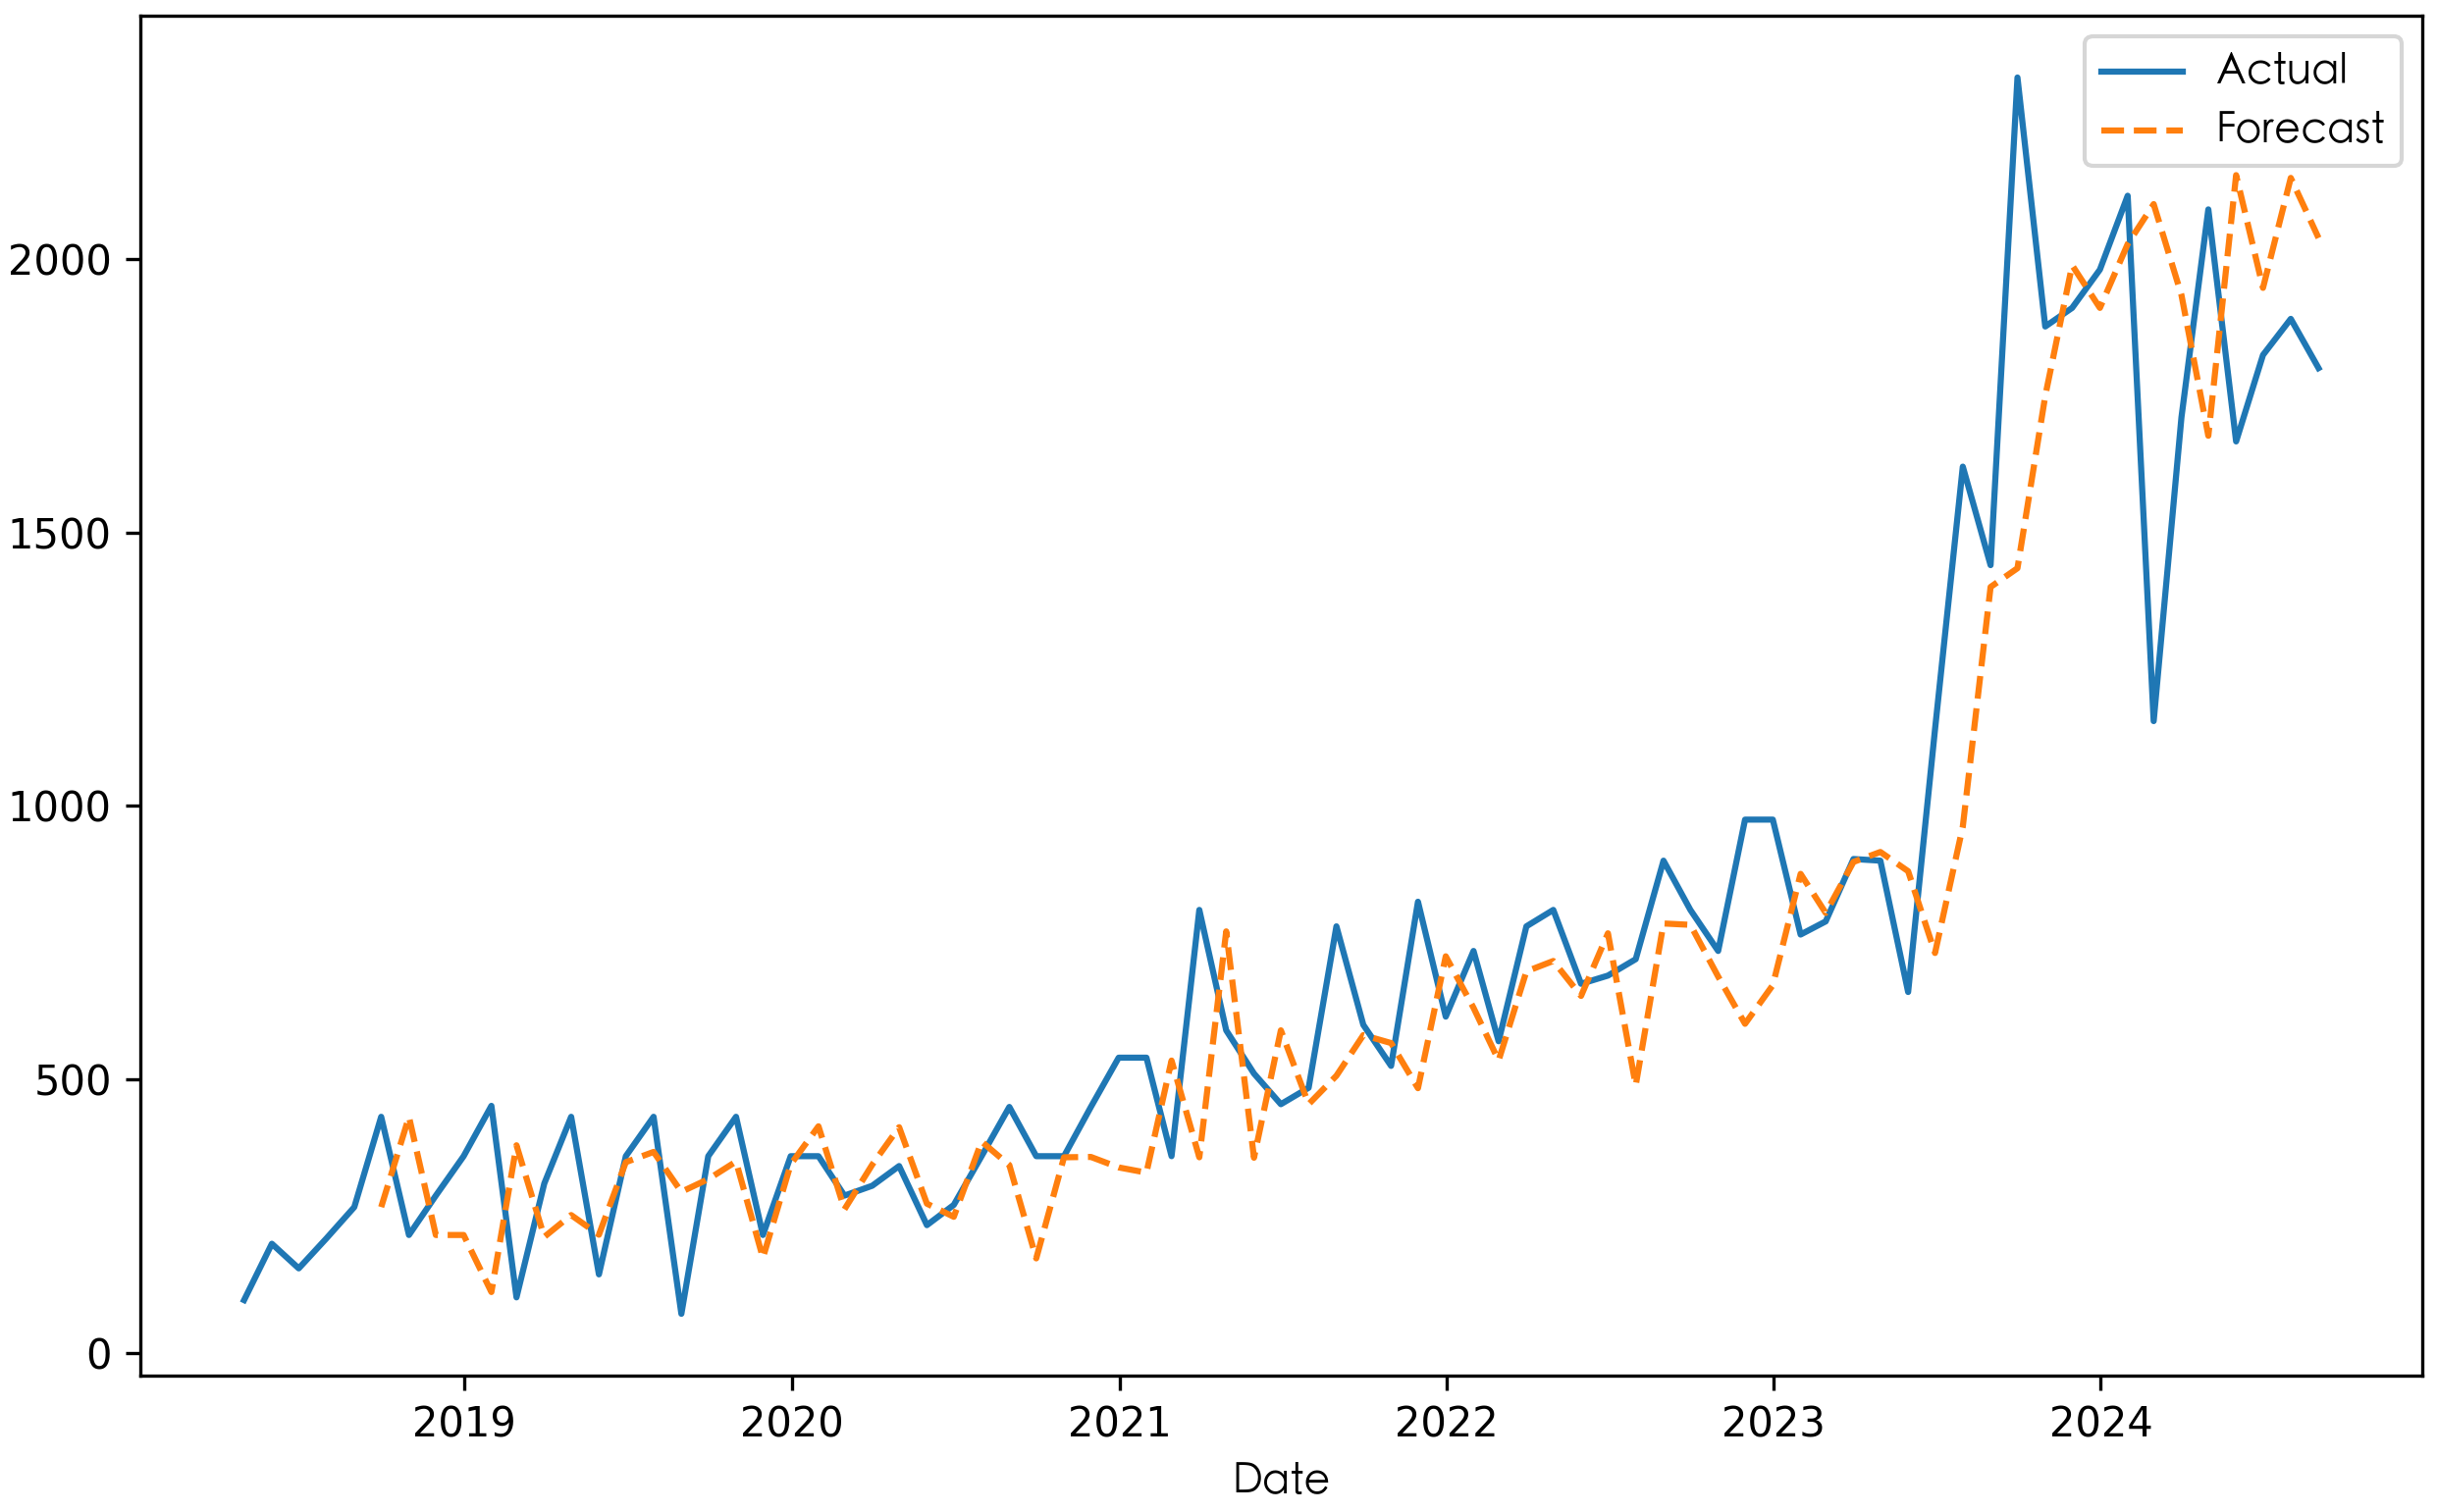
\includegraphics[width=\linewidth]{../Result_Paper/XGBoost_Prediction_麦考酚钠肠溶片_瑞士诺华.png}
\caption{DynamicXSP-X (XGBoost) Model Prediction for Mycophenolate Sodium Enteric Tablets by Novartis.}
\label{fig:mycophenolate}
\end{figure}
\item \textbf{Drug:} Flurbiprofen Gel Patch
\begin{itemize}
\item \textbf{Manufacturer:} Jingtaide
\item \textbf{Metrics:} $R^2 = 0.7902$, SMAPE = 21.14
\end{itemize}
DynamicXSP-X (XGBoost) Model effectively handled the increasing trend and high volatility in sales, demonstrating its strength in capturing complex patterns and sudden market changes.
\begin{figure}[H]
\centering
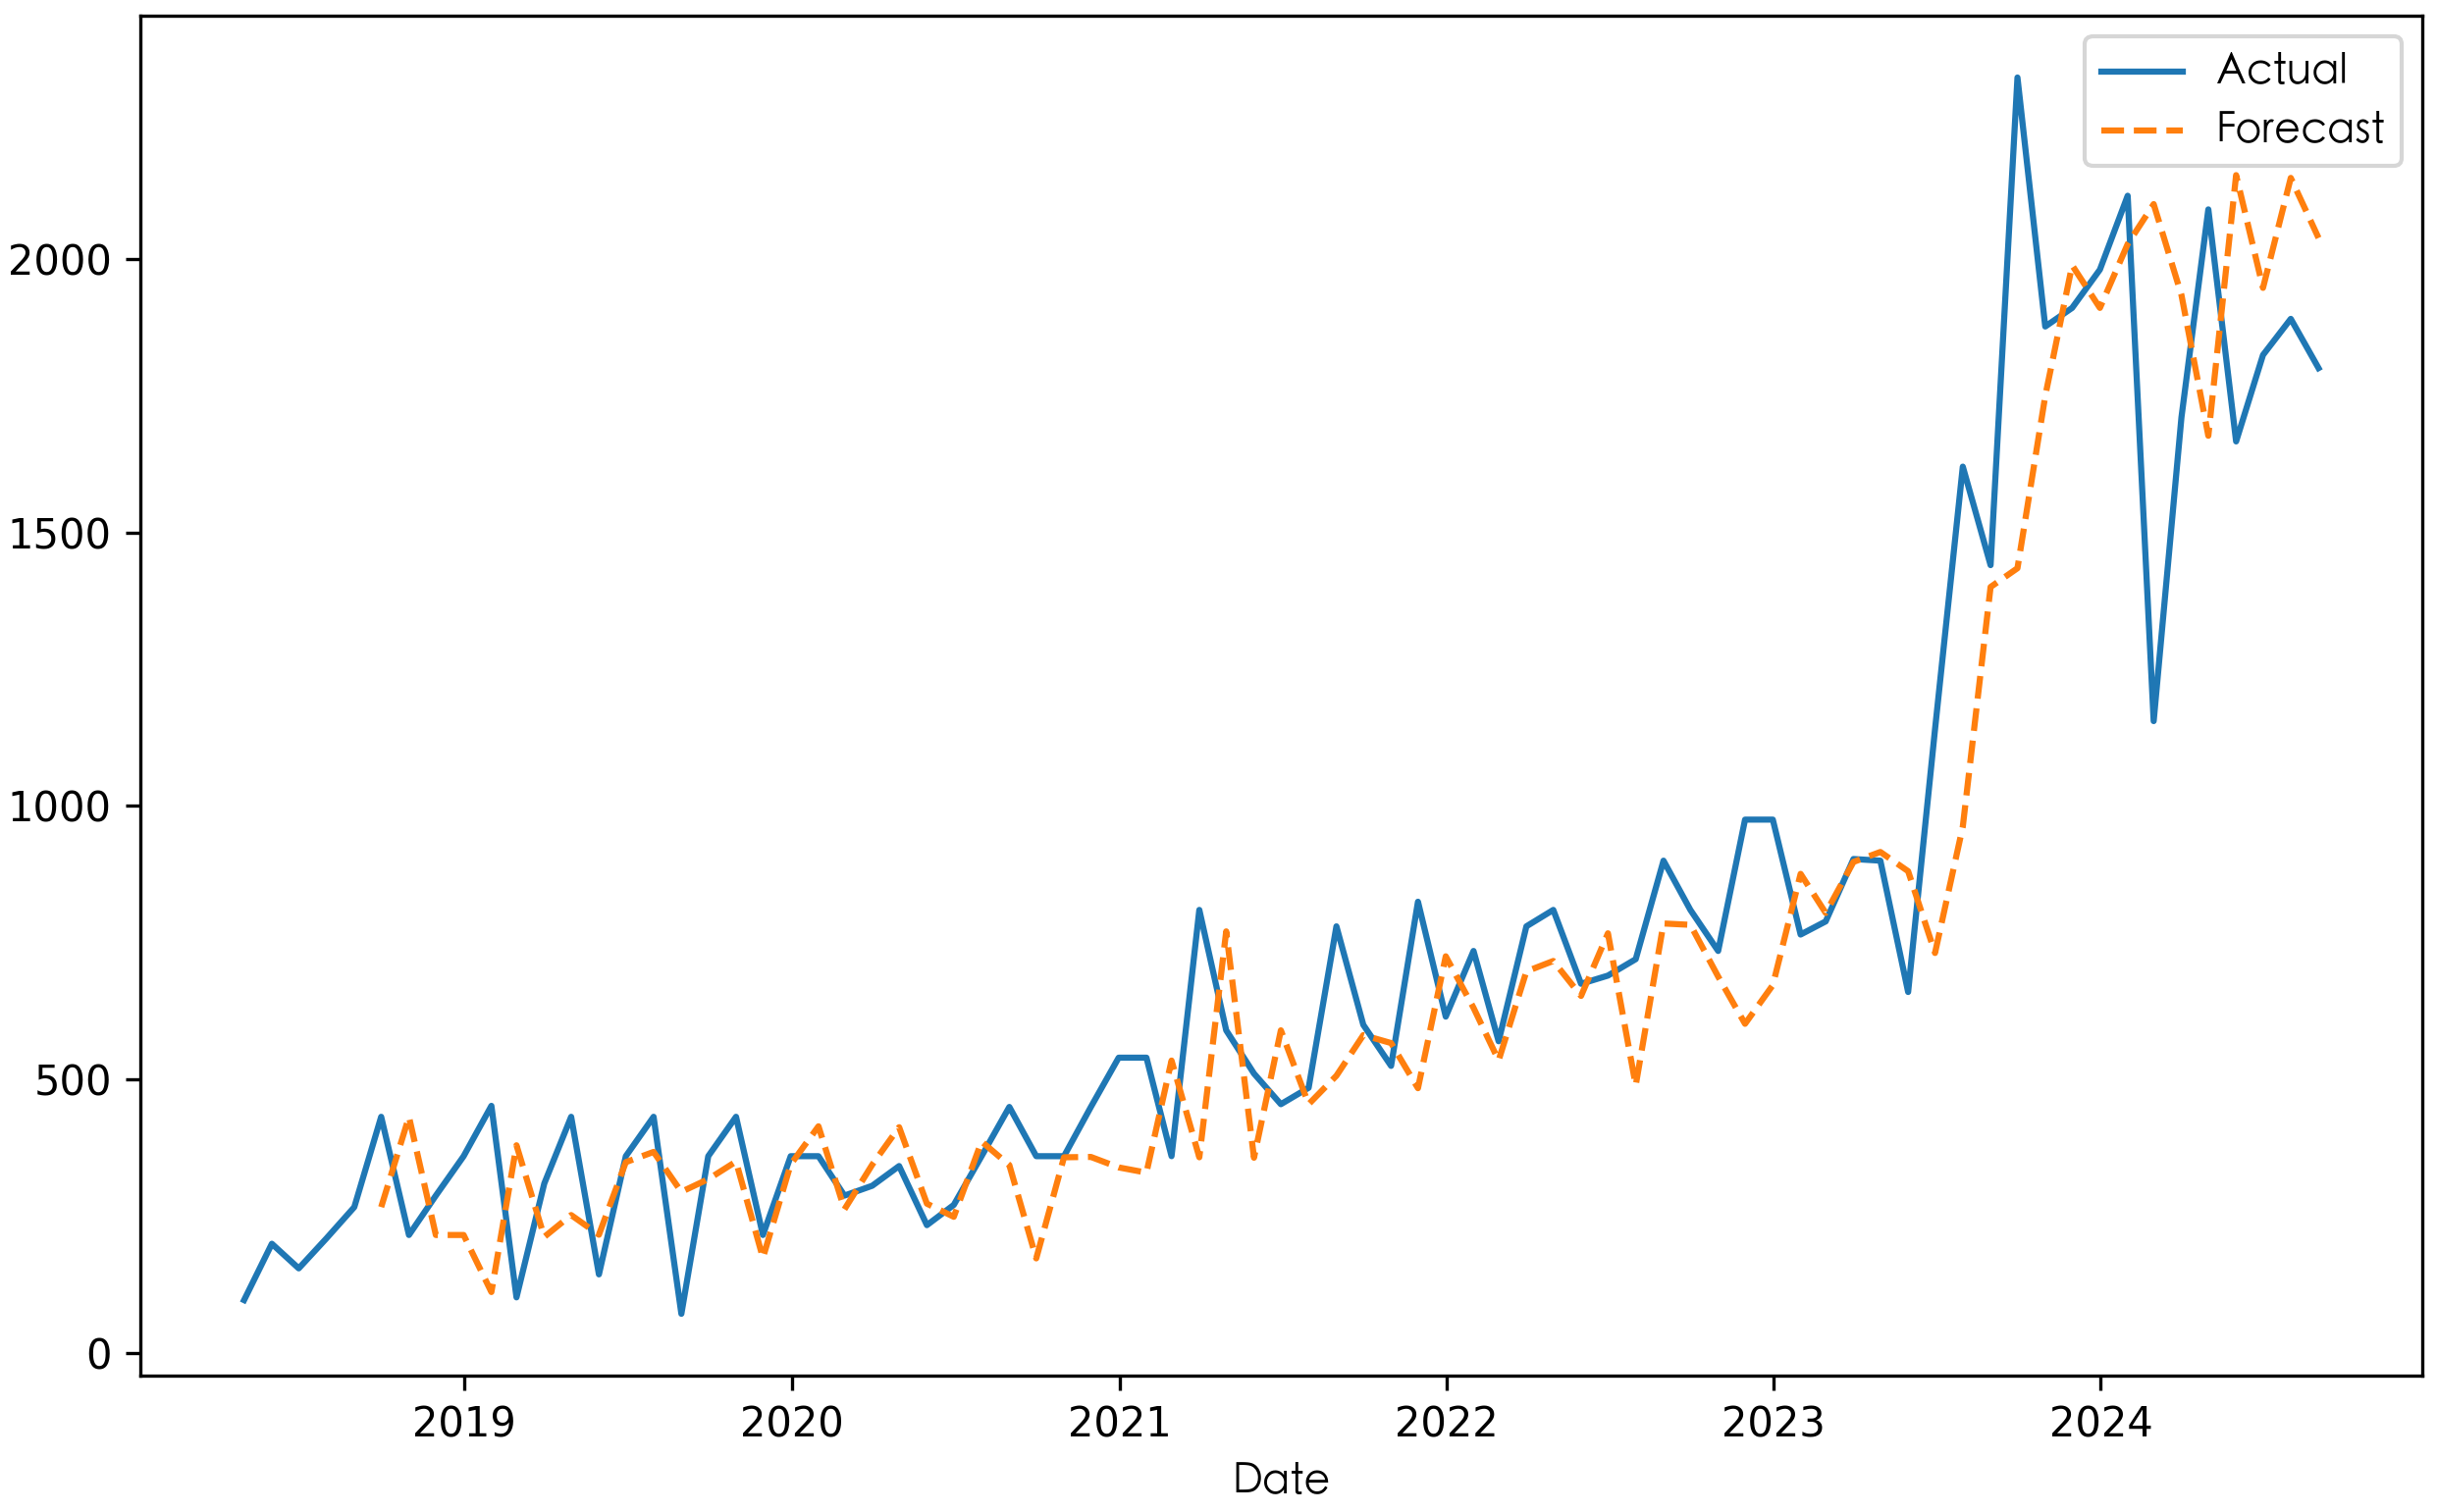
\includegraphics[width=\linewidth]{../Result_Paper/XGBoost_Prediction_麦考酚钠肠溶片_瑞士诺华.png}
\caption{DynamicXSP-X (XGBoost) Model Prediction for Flurbiprofen Gel Patch by Jingtaide.}
\label{fig:flurbiprofen}
\end{figure}
\end{itemize}

\paragraph{DynamicXSP-P (Prophet) Model}
\begin{itemize}
\item \textbf{Drug:} Compound Phellodendron Liquid
\begin{itemize}
\item \textbf{Manufacturer:} Lu Hanfang
\item \textbf{Metrics:} $R^2 = 0.7898$, SMAPE = 22.63
\end{itemize}
DynamicXSP-P (Prophet) Model excelled in modeling this drug's sales pattern due to its robust handling of trend changes and seasonal variations, particularly evident in the steady growth pattern.
\begin{figure}[H]
\centering
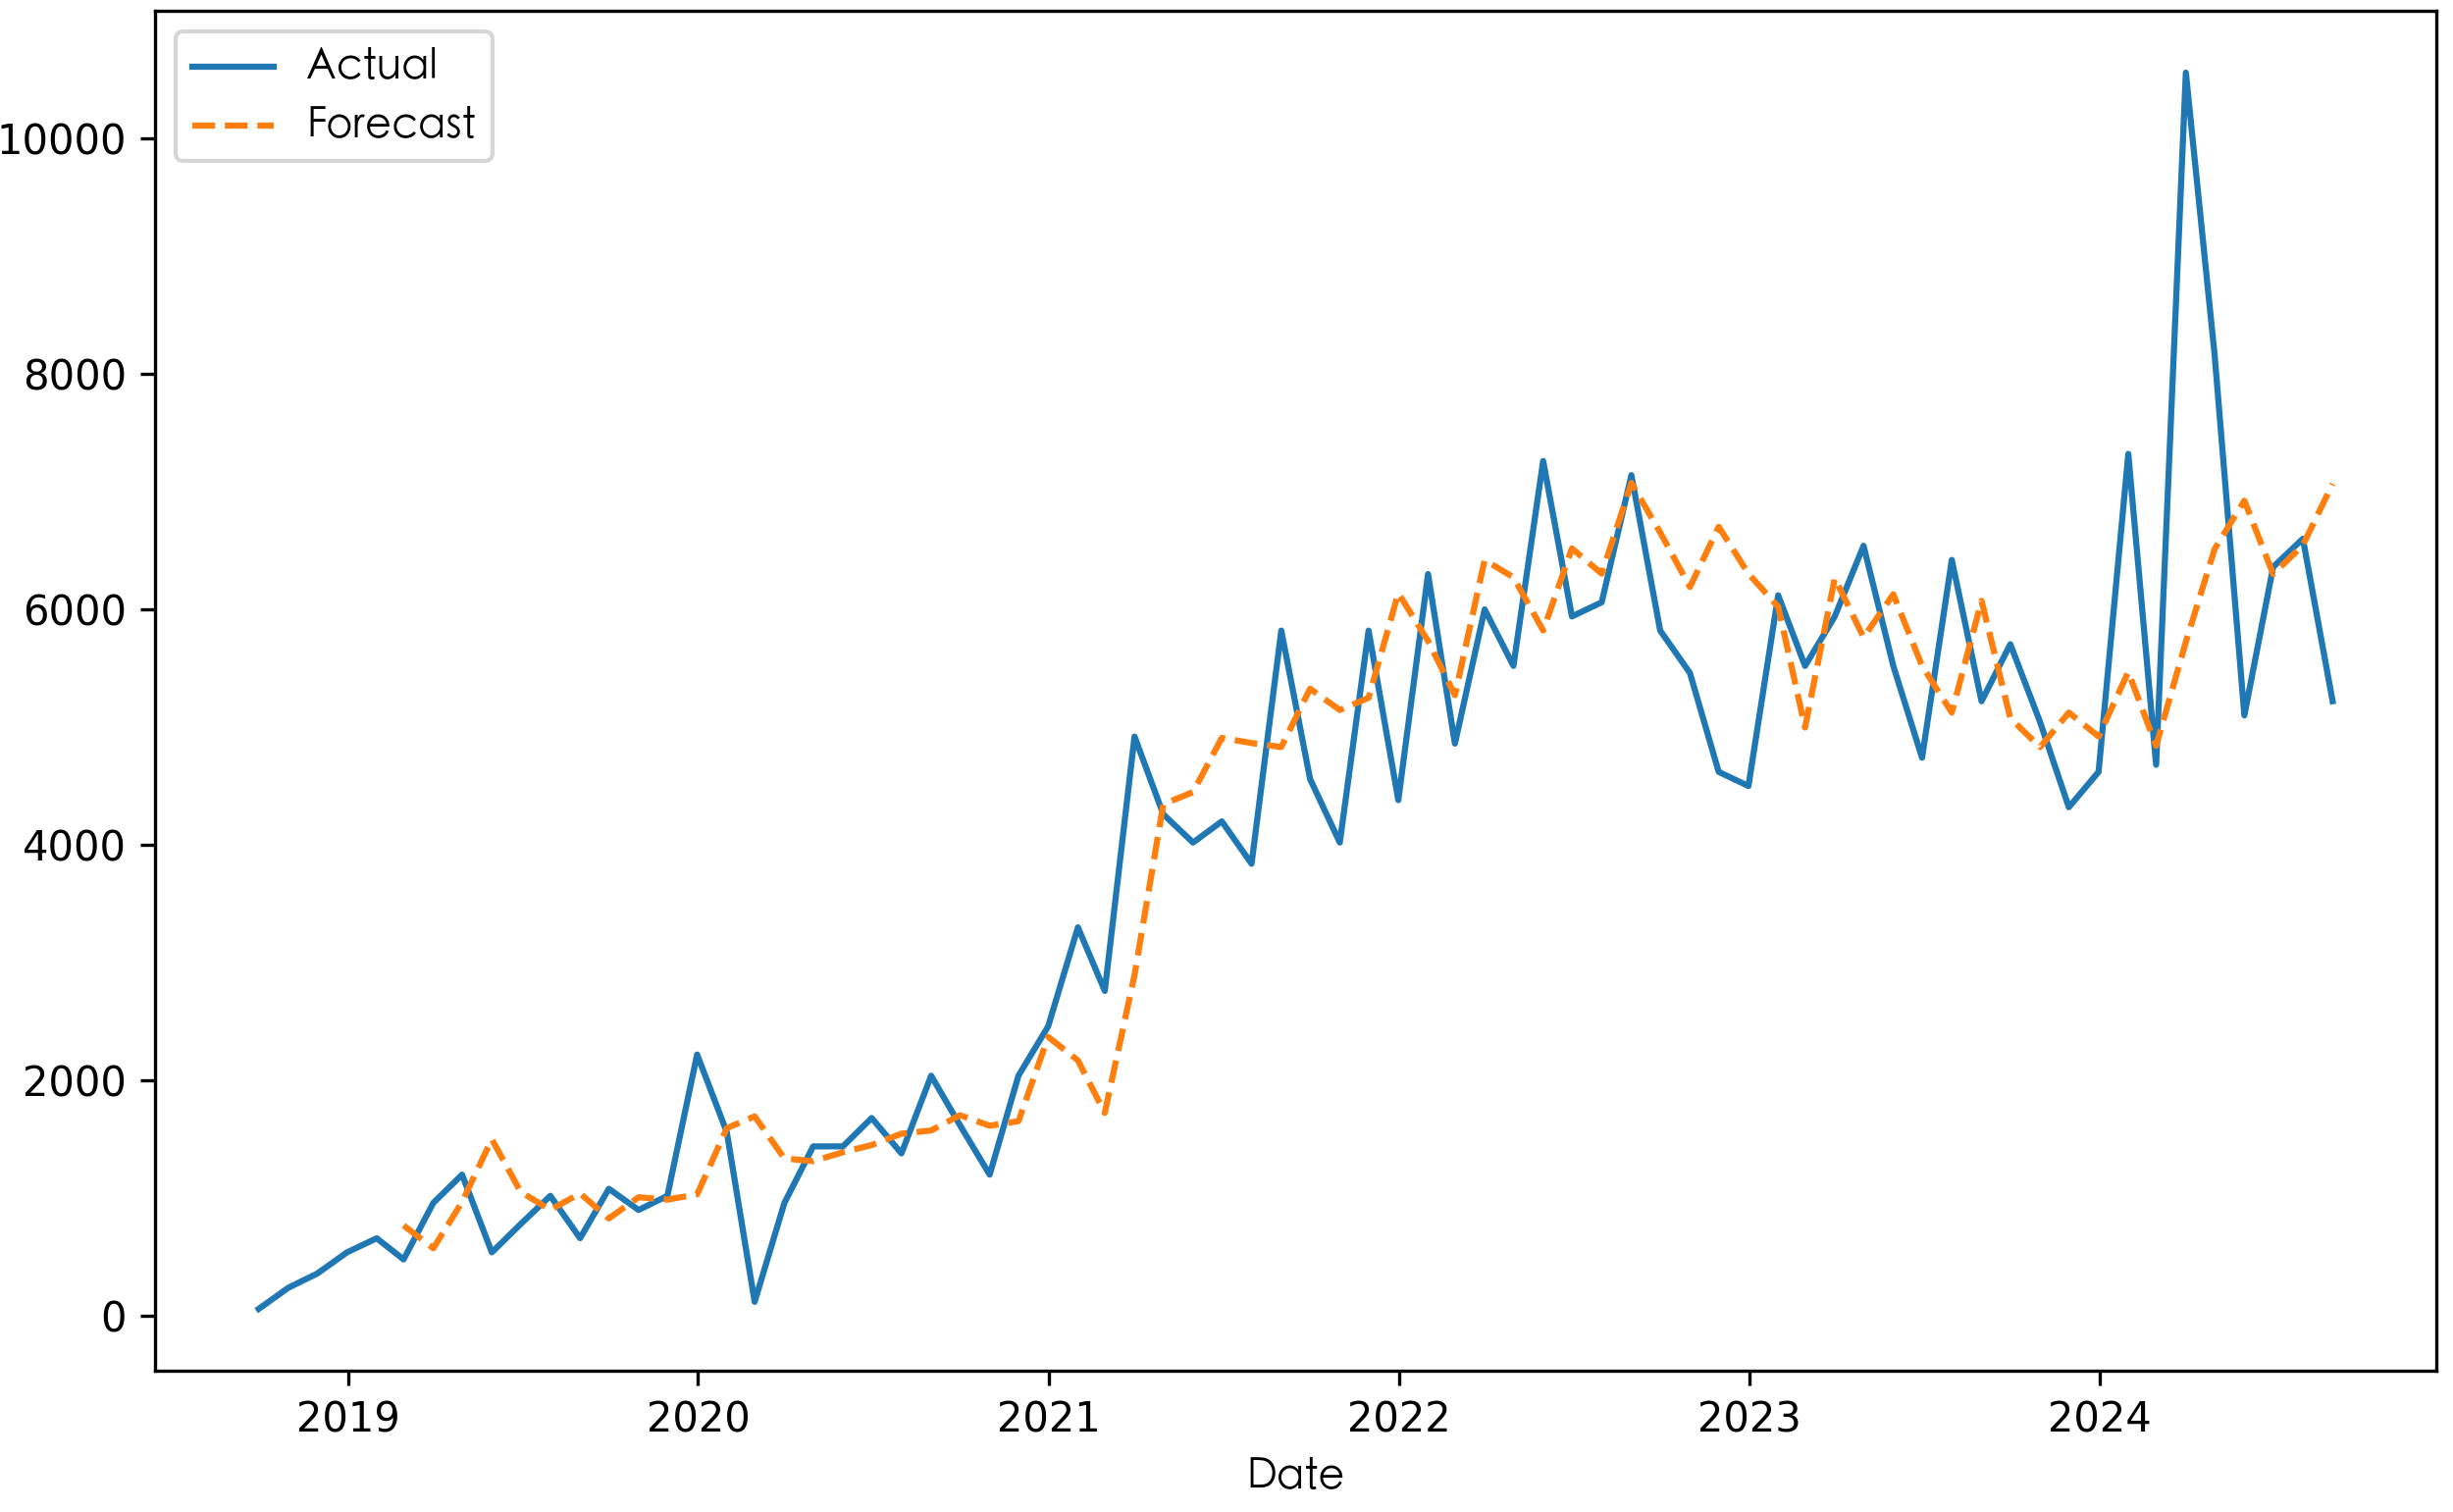
\includegraphics[width=\linewidth]{../Result_Paper/Prophet_Prediction_复方黄柏液涂剂_鲁汉方.png}
\caption{DynamicXSP-P (Prophet) Model Prediction for Compound Phellodendron Liquid by Lu Hanfang.}
\label{fig:phellodendron}
\end{figure}
\item \textbf{Drug:} Shenshuaining Tablets
\begin{itemize}
\item \textbf{Manufacturer:} Shanhaiguan Pharmaceutical
\item \textbf{Metrics:} $R^2 = 0.7348$, SMAPE = 21.86
\end{itemize}
DynamicXSP-P (Prophet) Model's capability to handle multiple seasonality levels and trend changes made it the optimal choice for this drug's complex sales pattern.
\begin{figure}[H]
\centering
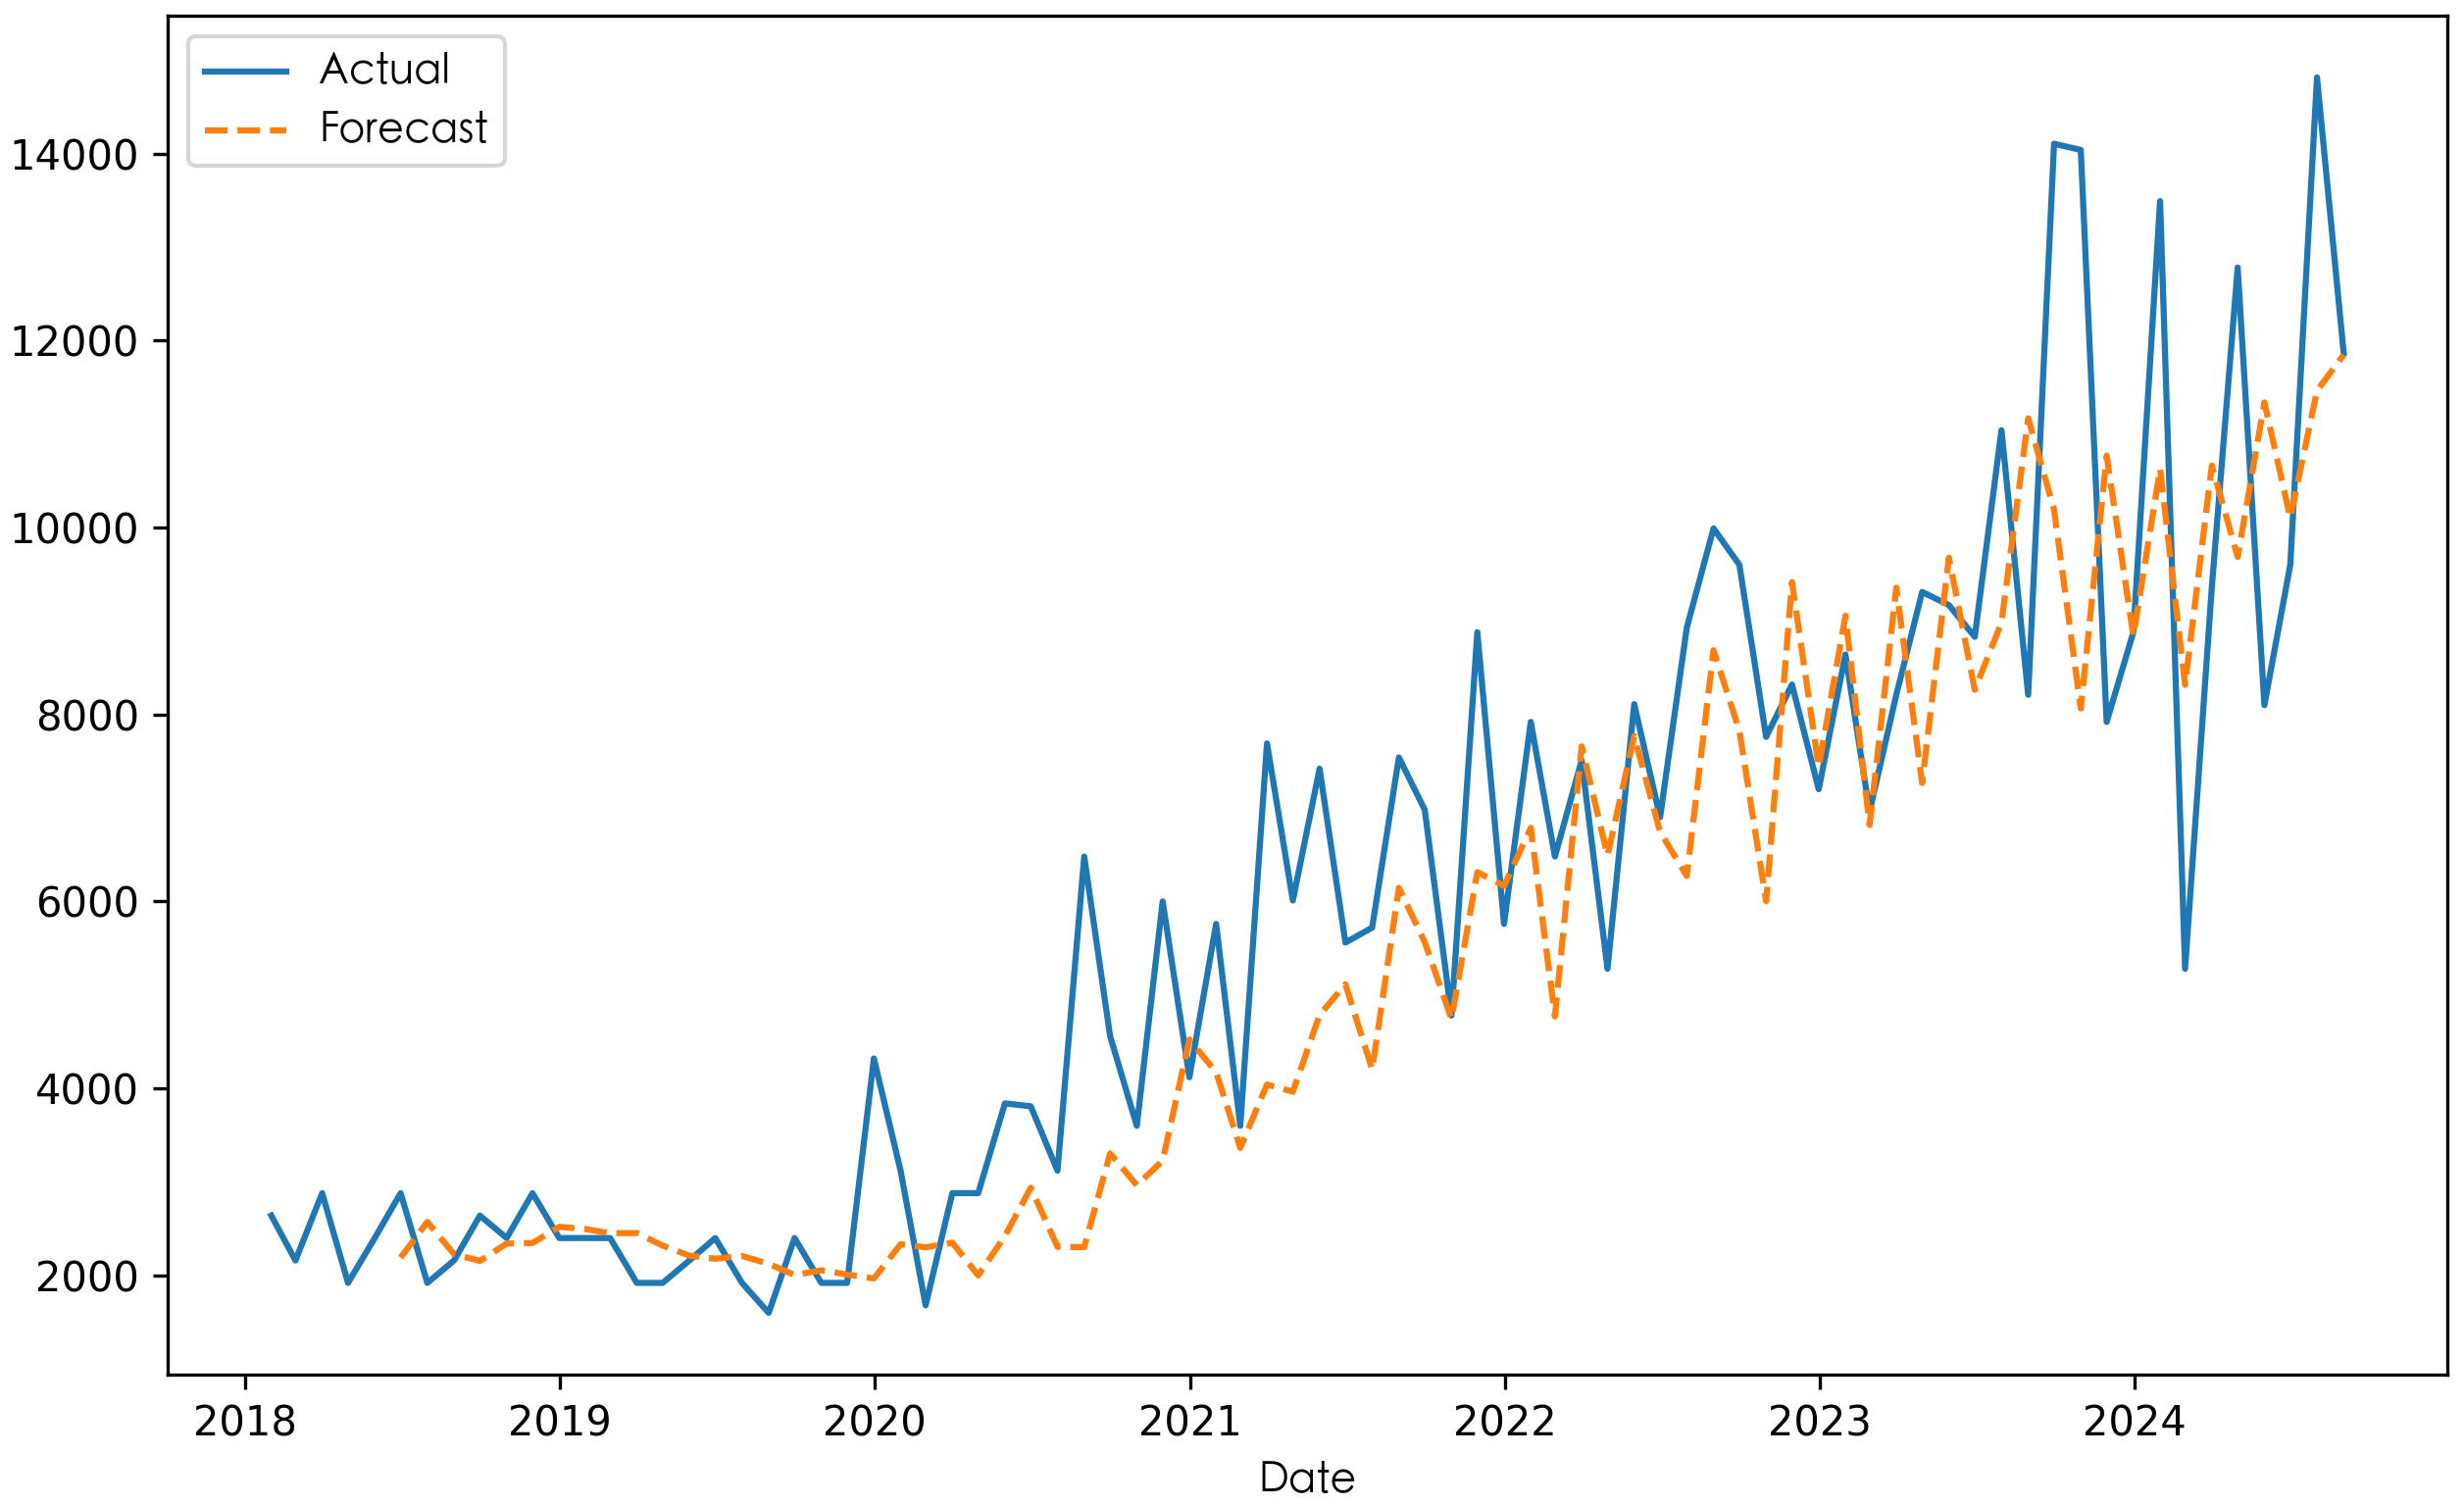
\includegraphics[width=\linewidth]{../Result_Paper/Prophet_Prediction_肾衰宁片_山海关药业.png}
\caption{DynamicXSP-P (Prophet) Model Prediction for Shenshuaining Tablets by Shanhaiguan Pharmaceutical.}
\label{fig:shenshuaining}
\end{figure}
\end{itemize}

\paragraph{DynamicXSP-S (SARIMAX) Model}
\begin{itemize}
\item \textbf{Drug:} Peritoneal Dialysis Solution [Lactate]
\begin{itemize}
\item \textbf{Manufacturer:} Huaren
\item \textbf{Metrics:} $R^2 = 0.8109$, SMAPE = 32.49
\end{itemize}
DynamicXSP-S (SARIMAX) Model demonstrated superior performance for this drug due to its ability to capture both the seasonal patterns and the gradual decline in demand shown in the time series. The model effectively handled the relatively stable periodic fluctuations until the sharp decline in 2023.
\begin{figure}[H]
\centering
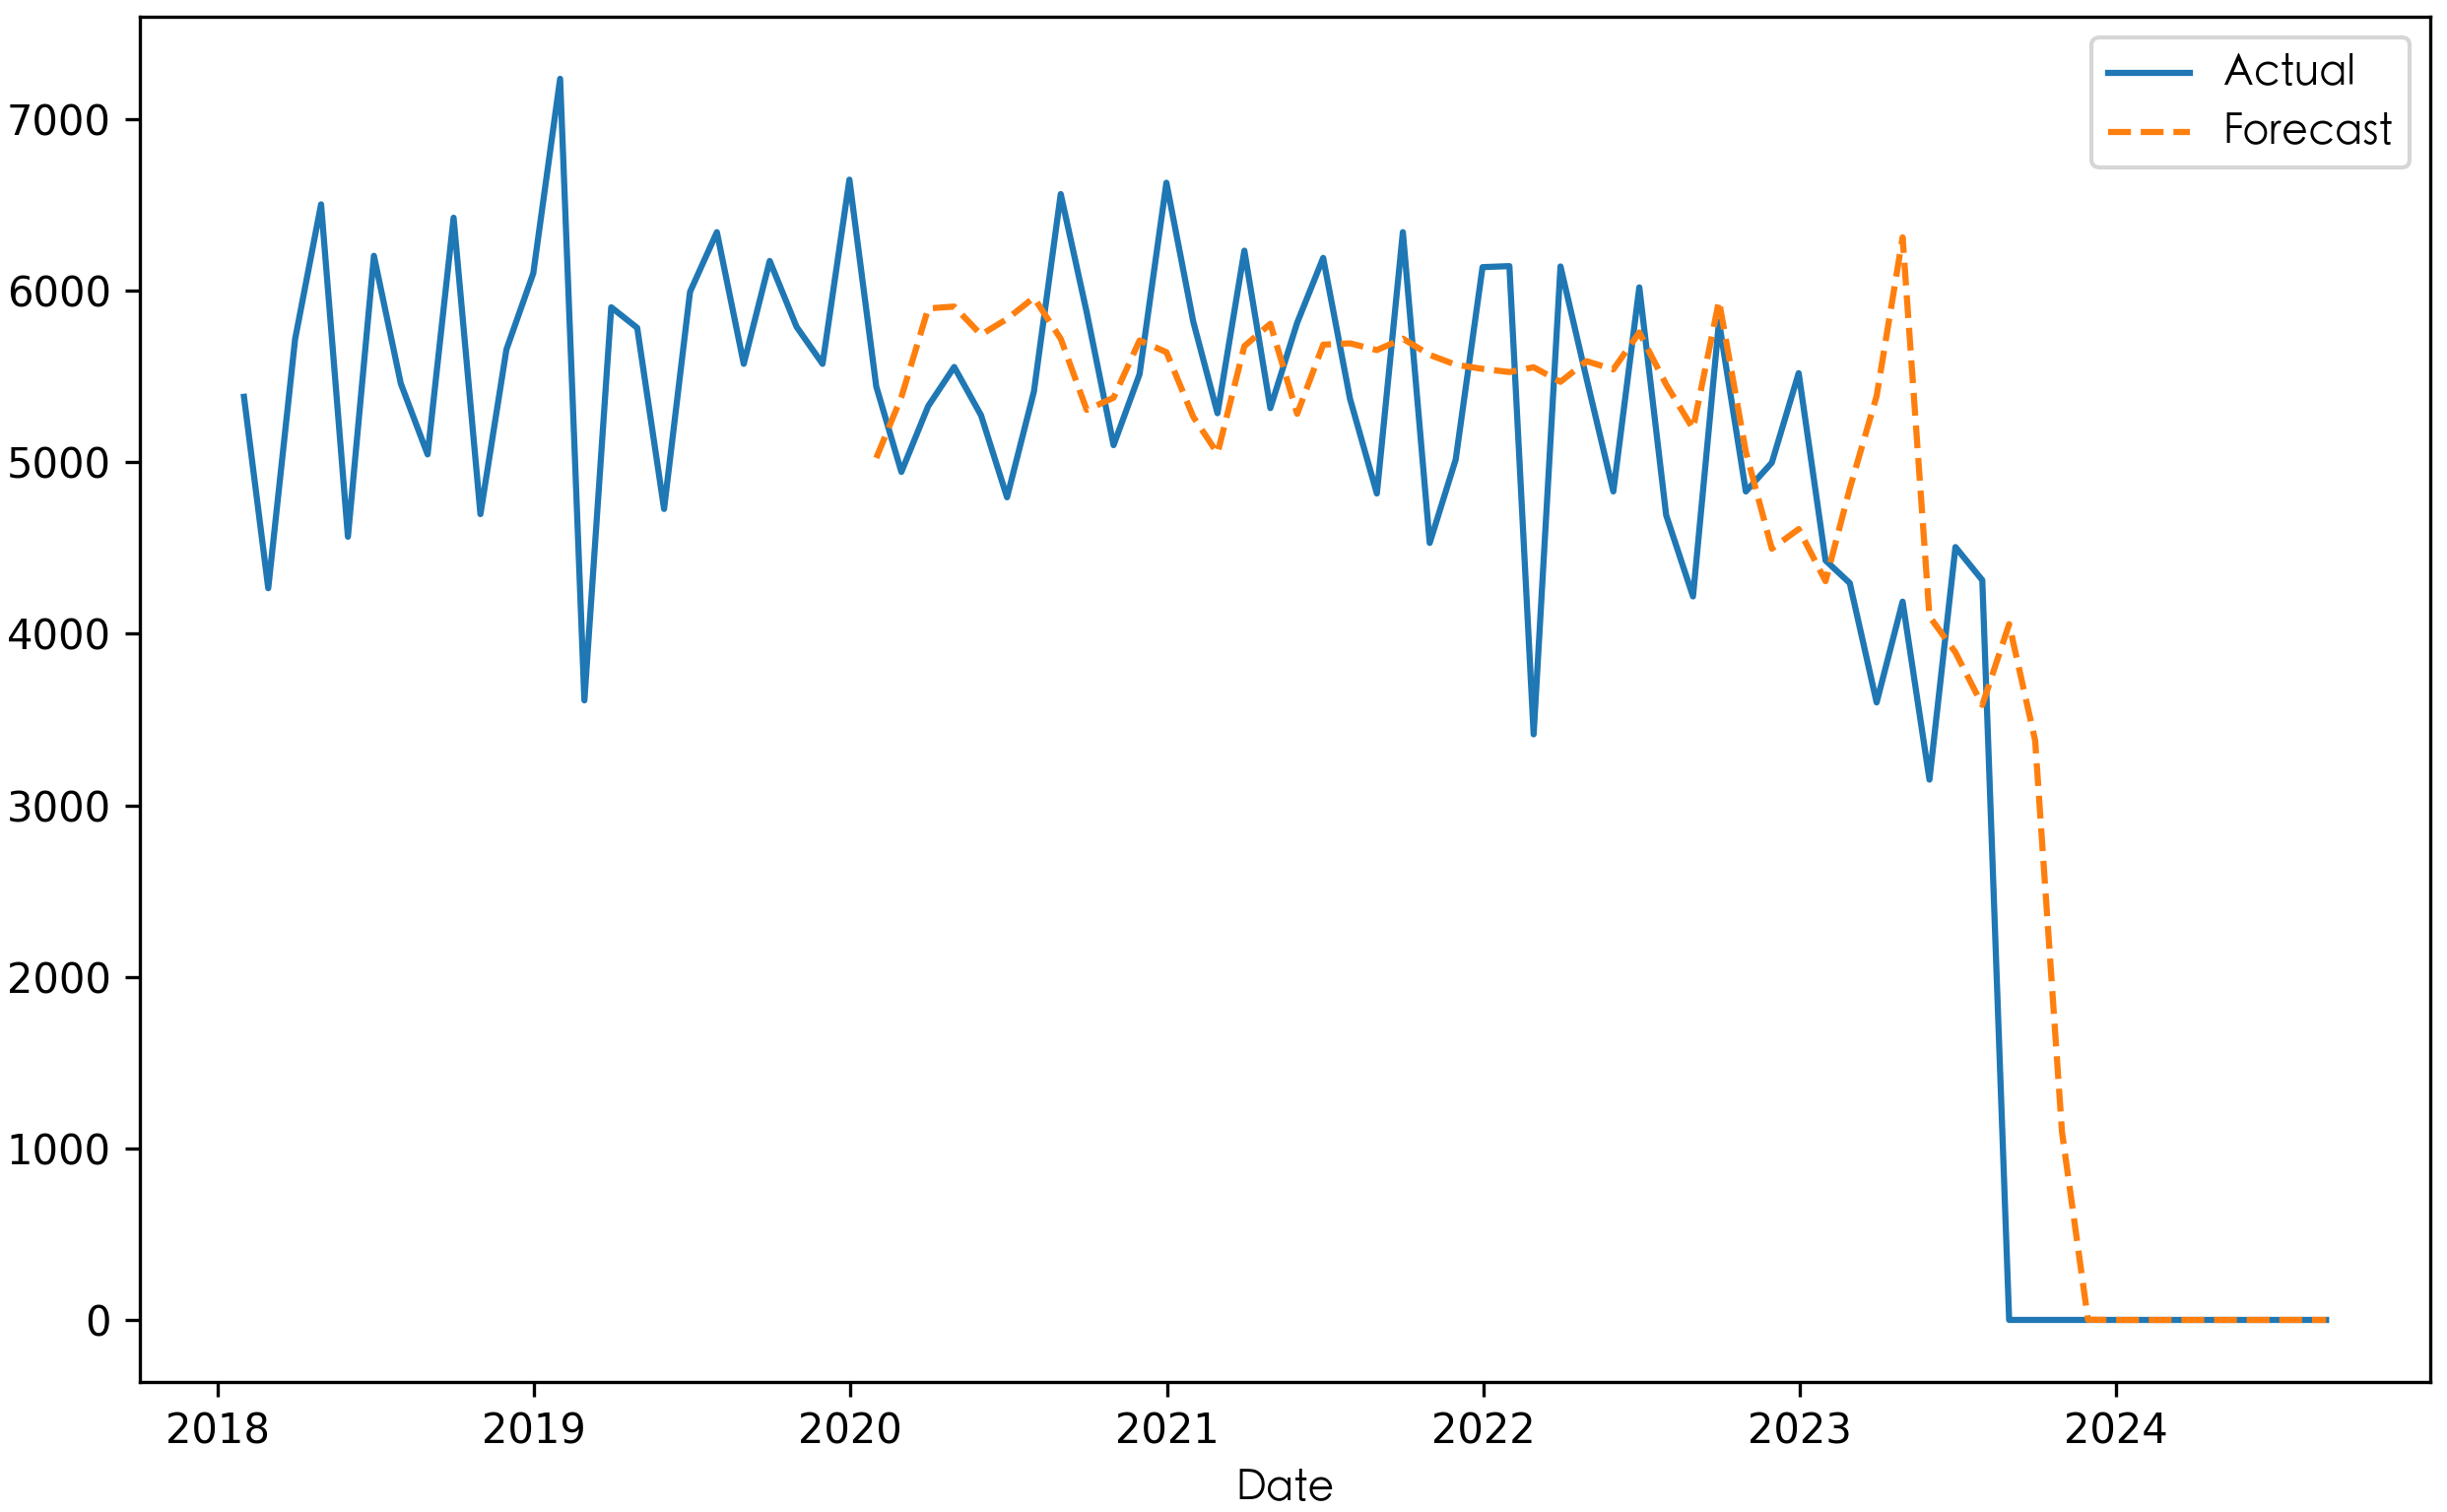
\includegraphics[width=\linewidth]{../Result_Paper/SARIMAX_Prediction_腹膜透析液[乳酸盐]_华仁.png}
\caption{DynamicXSP-S (SARIMAX) Model Prediction for Peritoneal Dialysis Solution by Huaren.}
\label{fig:peritoneal}
\end{figure}
\item \textbf{Drug:} Vitamin B1 Tablets
\begin{itemize}
\item \textbf{Manufacturer:} Xinyi Huanghe
\item \textbf{Metrics:} $R^2 = 0.7345$, SMAPE = 35.37
\end{itemize}
DynamicXSP-S (SARIMAX) Model was effective for this drug due to its ability to handle the external influences and volatility in the sales data.
\begin{figure}[H]
\centering
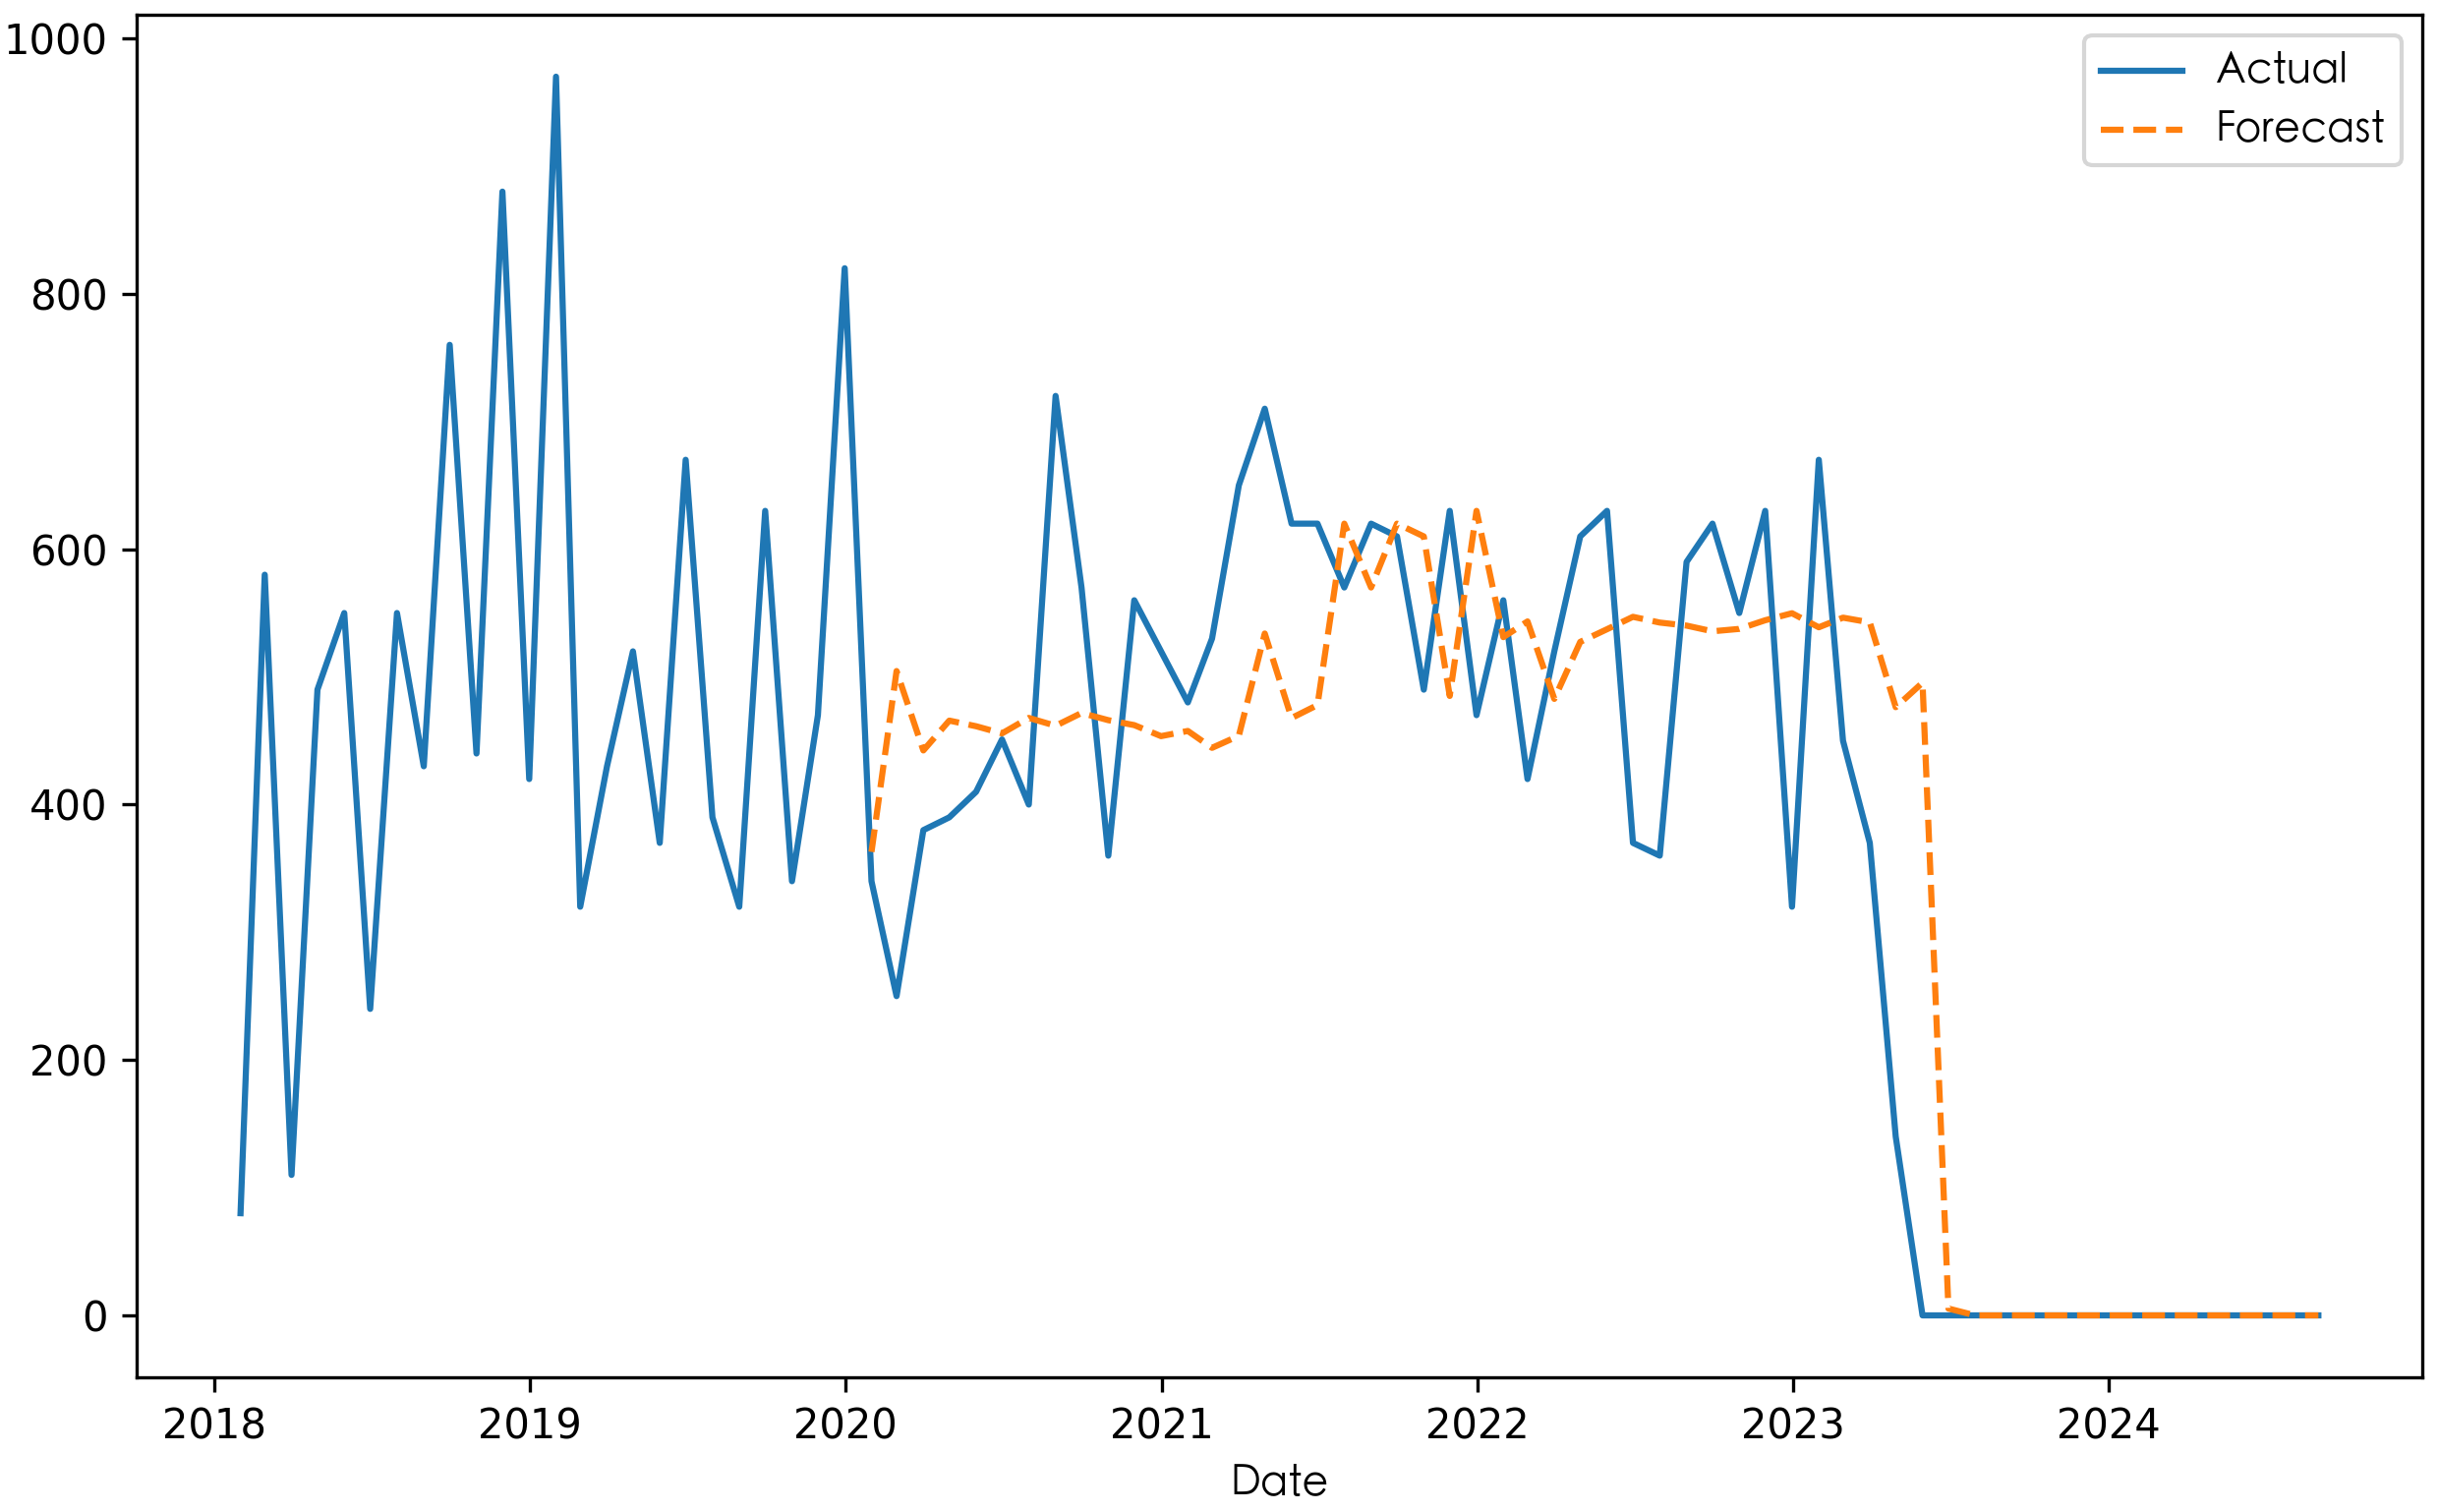
\includegraphics[width=\linewidth]{../Result_Paper/SARIMAX_Prediction_维生素B1片_信谊黄河.png}
\caption{DynamicXSP-S (SARIMAX) Model Prediction for Vitamin B1 Tablets by Xinyi Huanghe.}
\label{fig:vitaminb1}
\end{figure}
\end{itemize}

\subsubsection{Overall Results}

The results highlighted that no single model universally outperformed the others across all cases, underscoring the importance of tailoring each choice of forecasting models to specific data characteristics. DynamicXSP-S (SARIMAX) Model presented superior capability in capturing seasonality influenced by external variables, such as pricing trends and policy changes. DynamicXSP-X (XGBoost) Model excelled in modeling complex, non-linear relationships within the data, making it particularly effective for patterns with high variability. DynamicXSP-P (Prophet) Model performed well in cases with dominant seasonality and long-term trends, such as periodic spikes in drug demand. These findings prove the necessary of DynamicXSP by leveraging the complementary strengths of each single model. 

The DynamicXSP model analysis reveals several key findings:

\textbf{Long-term Trend Capture}:
\begin{itemize}
\item All models effectively captured the underlying growth trends, with Prophet showing particular strength in long-term pattern recognition.
\item DynamicXSP-S (SARIMAX) Model demonstrated superior performance in capturing gradual trend changes, as evidenced in the insulin device forecasts.
\end{itemize}

\textbf{Seasonal Pattern Recognition}:
\begin{itemize}
\item DynamicXSP-X (XGBoost) Model effectively captured complex seasonal patterns in chronic medication usage.
\item DynamicXSP-S (SARIMAX) Model showed strong performance in regular seasonal variations, particularly in established products.
\end{itemize}

\textbf{Growth Pattern Adaptation}:
\begin{itemize}
\item DynamicXSP-P (Prophet) Model demonstrated superior capability in adapting to emerging growth patterns.
\item DynamicXSP-X (XGBoost) Model showed strong performance in capturing non-linear growth relationships.
\end{itemize}

\subsection{Comparison with Basic Models}

To demonstrate the effectiveness of the DynamicXSP model, we compare it against three baseline models: Prophet, SARIMAX, and XGBoost, each applied without optimizations such as hyperparameter tuning, rolling predictions, or grid search.

The results indicate the baseline models are hard to provide accurate predictions. Compared with DynamicXSP, SMAPE values are notably higher in the baseline models across all cases. Additionally, the baseline models show limited explanatory power, which means an adaptive approach is necessary. Therefore, the DynamicXSP model, which incorporates rolling forecasting, parameter tuning, and additional feature engineering, exhibits significantly improved performance. 

\section{Conclusion and Future Work}

\subsection{Conclusion}

This study presents the effectiveness and adaptability of the DynamicXSP framework in addressing the challenges of pharmaceutical demand forecasting. By integrating the complementary strengths of SARIMAX, Prophet, and XGBoost, along with advanced techniques such as rolling-window forecasting, grid search and feature engineering, DynamicXSP model provides a robust solution for predicting drug consumption across diverse drug-manufacturer combinations.

This framework's tailored approach allows the selection and integration of models based on the specific characteristics of each dataset, enabling it to overcome limitations inherent in single-model approaches. The performance evaluation highlights the key contributions of each model within the framework:

\begin{itemize} 
    \item \textbf{DynamicXSP-X (XGBoost) Model}: Demonstrates superior handling of nonlinear relationships, particularly excelling in short-term predictions, where it outperformed SARIMAX and Prophet in terms of RMSE and SMAPE. 
    \item \textbf{DynamicXSP-S (SARIMAX) Model}: Performs well in datasets with seasonal trends and where external (exogenous) variables like pricing or policy changes, playing an significant role. 
    \item \textbf{DynamicXSP-P (Prophet) Model}: Effectively captures long-term seasonality and trends, proving valuable for datasets with prominent periodic patterns, although it faces challenges with sparsity. \end{itemize}

The DynamicXSP framework is able to dynamically adapt to various data characteristics and leverage the complementary strengths of multiple models, which highlights its practicality and scalability. This hybrid approach not only improves the accuracy and robustness but also lays a foundation for wider applications of drug consumption forecasting.

\subsection{Limitations and Future Work}
To some extent, The DynamicXSP framework has some limitations that the selection of external variables remains largely domain-driven, and the model may benefit from a more systematic approach to identifying relevant exogenous factors. 

To further improve drug inventory predictions, we propose the following future research directions. 
\begin{itemize}
    \item \textbf{Hybrid Framework Expansion}: Expand the hybrid framework by incorporating other models, such as LightGBM, Transformer-based architectures and ensemble methods to capture both short-term fluctuations and long-term trends.
    \item \textbf{External Variable Enrichment}: Explore additional exogenous variables such as patient inflow, epidemic outbreak data, seasonal illnesses (e.g., flu seasons), or hospital-specific factors from systematic approach to improve prediction accuracy.
    \item \textbf{Automated Model Selection}: Implement automated hyperparameter tuning and model selection techniques (e.g., Bayesian optimization) to improve forecasting performance with minimal manual intervention.
\end{itemize}

By addressing these areas, the proposed framework can become a more robust and scalable solution for hospital pharmacy inventory management, ensuring operational efficiencies of hospital pharmacies.

\begin{thebibliography}{99}

    \bibitem{koala2021factors} 
    D. Koala, Z. Yahouni, G. Alpan, and Y. Frein, “Factors influencing drug consumption and prediction methods,” in \textit{CIGI-Qualita: Conférence Internationale Génie Industriel QUALITA}, Grenoble, France, 2021.
    
    \bibitem{taylor2018forecasting}
    S. J. Taylor and B. Letham, “Forecasting at scale,” \textit{The American Statistician}, vol. 72, no. 1, pp. 37–45, 2018.

    \bibitem{chen2016xgboost}
    T. Chen and C. Guestrin, “XGBoost: A scalable tree boosting system,” \textit{Proceedings of the 22nd ACM SIGKDD International Conference on Knowledge Discovery and Data Mining}, 2016, pp. 785–794.

    \bibitem{meng2021comparative}
    J. Meng, Q. Zhang, and X. Li, “Comparative analysis of Prophet and LSTM models in drug sales forecasting,” \textit{Journal of Physics: Conference Series}, vol. 1910, no. 1, p. 012059, 2021.

    \bibitem{xu2019hybrid}
    W. Xu, Y. Wang, and J. Zhao, “A hybrid modelling method for time series forecasting based on a linear regression model and deep learning,” \textit{Applied Intelligence}, vol. 49, no. 7, pp. 2875–2888, 2019.

    \bibitem{siddiqui2021hybrid}
    R. Siddiqui, A. Khan, and M. Ahmed, “A Hybrid Demand Forecasting Model for Greater Forecasting Accuracy: The Case of the Pharmaceutical Industry,” \textit{Supply Chain Forum: An International Journal}, vol. 22, no. 3, pp. 1–13, 2021.

    \bibitem{rathipriya2022pharma}
    R. Rathipriya, M. Saranya, and K. Ramkumar, “Demand Forecasting Model for Time-Series Pharmaceutical Data Using Neural Networks,” \textit{Neural Computing and Applications}, vol. 35, pp. 1945–1957, 2022.

\end{thebibliography}

\raggedbottom  % 允许页面填充不均匀,减少空白

\appendix
\section{Sample Selection Algorithm}
\label{appendix:sample-selection}

The following pseudocode outlines the sample selection process used to ensure the quality and relevance of the dataset for modeling tasks:

\begin{algorithm}[H]
\caption{Sample Selection Algorithm}
\begin{algorithmic}[1]
\Require Cleaned data $df$, configuration thresholds $\text{config}$
\Ensure Filtered dataset $final\_df$
\State $final\_df \gets \emptyset$
\For{each unique combination of drug name and manufacturer $(d, m)$ in $df$}
    \State $group\_data \gets$ subset of $df$ for $(d, m)$
    \If{length of $group\_data < \text{config.min\_months}$ \textbf{or} sum of consumption $= 0$}
        \State \textbf{Skip group} \Comment{Insufficient or sparse data}
    \EndIf
    \State $non\_zero\_ratio \gets$ proportion of non-zero consumption in $group\_data$
    \If{$non\_zero\_ratio < \text{config.sparsity\_threshold}$}
        \State \textbf{Skip group} \Comment{Data too sparse}
    \EndIf
    \State $acf\_values \gets$ autocorrelation function of consumption in $group\_data$
    \If{$\max(acf\_values[1:]) < \text{config.min\_acf\_threshold}$}
        \State \textbf{Skip group} \Comment{Insufficient autocorrelation}
    \EndIf
    \If{no start date $\geq \text{config.min\_start\_date}$ in $group\_data$}
        \State \textbf{Skip group} \Comment{No recent data}
    \EndIf
    \State $variance \gets$ variance of consumption in $group\_data$
    \If{$variance < \text{config.min\_variance\_threshold}$}
        \State \textbf{Skip group} \Comment{Variance too low}
    \EndIf
    \State $missing\_ratio \gets$ maximum missing ratio for features in $group\_data$
    \If{$missing\_ratio > \text{config.max\_missing\_ratio}$}
        \State \textbf{Skip group} \Comment{Feature missing data too high}
    \EndIf
    \State $skewness \gets$ skewness of consumption in $group\_data$
    \If{$|skewness| > \text{config.max\_skewness}$}
        \State \textbf{Skip group} \Comment{Target variable too skewed}
    \EndIf
    \State $correlation \gets$ correlation of consumption with lagged features in $group\_data$
    \If{$|correlation| < \text{config.min\_correlation}$}
        \State \textbf{Skip group} \Comment{Insufficient correlation with features}
    \EndIf
    \State $final\_df \gets final\_df \cup group\_data$
\EndFor
\State \Return $final\_df$
\end{algorithmic}
\end{algorithm}

\bibliographystyle{IEEEtran}
\bibliography{references}
\end{document}

